% Conference Talk Template Sample
% 会议演讲模板样板
% 适用于：学术会议、技术峰会、TED风格演讲、闪电演讲

\documentclass[aspectratio=169,11pt]{beamer}

% ========== 基础包 ==========
\usepackage[fontset=fandol,space=true,scheme=plain]{ctex}
\usetheme{metropolis}

% ========== 额外包 ==========
\usepackage{graphicx}
\usepackage{booktabs}
\usepackage{amsmath}
\usepackage{tikz}
\usetikzlibrary{shapes,arrows,positioning,calc}
\usepackage{pgfplots}
\pgfplotsset{compat=1.18}

% ========== 自定义颜色 ==========
\definecolor{primary}{RGB}{0,102,204}
\definecolor{accent}{RGB}{255,102,0}
\definecolor{success}{RGB}{0,153,51}

% ========== 文档信息 ==========
\title{\textbf{基于深度学习的图像识别技术}}
\subtitle{从理论到实践的突破}
\author{演讲者姓名}
\institute{XX实验室 / XX公司}
\date{2024年技术峰会}

% ========== 开始文档 ==========
\begin{document}

% ---------- 封面 ----------
\begin{frame}
    \titlepage
\end{frame}

% ---------- 自我介绍（可选） ----------
\begin{frame}{关于我}
    \begin{columns}[T]
        \begin{column}{0.35\textwidth}
            \centering
            \begin{tikzpicture}
                \node[circle,draw,minimum size=3cm,fill=primary!20] {头像/Logo};
            \end{tikzpicture}
        \end{column}
        \begin{column}{0.60\textwidth}
            \textbf{演讲者：XXX}
            \begin{itemize}
                \item XX大学计算机科学博士
                \item 前 XX 公司 AI 研究员
                \item 专注领域：计算机视觉、深度学习
                \item GitHub: @username
            \end{itemize}
            
            \vspace{0.5em}
            \textbf{团队：XX 实验室}\\
            致力于推动 AI 技术落地应用
        \end{column}
    \end{columns}
\end{frame}

% ---------- 问题背景 ----------
\begin{frame}{问题背景：图像识别的挑战}
    \begin{columns}[T]
        \begin{column}{0.55\textwidth}
            \textbf{传统方法的局限：}
            \begin{itemize}
                \item 手工特征设计耗时耗力
                \item 对复杂场景泛化能力差
                \item 无法处理大规模数据
                \item 准确率遇到瓶颈（80-85\%）
            \end{itemize}
            
            \vspace{0.5em}
            \textbf{实际应用需求：}
            \begin{itemize}
                \item 医疗影像诊断（准确率需 > 95\%）
                \item 自动驾驶实时识别（延迟 < 50ms）
                \item 工业质检（处理速度 > 100fps）
            \end{itemize}
        \end{column}
        \begin{column}{0.42\textwidth}
            \centering
            \begin{tikzpicture}[scale=0.7]
                \node[draw,fill=red!20,minimum width=3cm,minimum height=1cm] at (0,3) {复杂背景};
                \node[draw,fill=red!20,minimum width=3cm,minimum height=1cm] at (0,1.5) {光照变化};
                \node[draw,fill=red!20,minimum width=3cm,minimum height=1cm] at (0,0) {遮挡模糊};
                \draw[->,thick] (1.5,3) -- (3,2.25);
                \draw[->,thick] (1.5,1.5) -- (3,2);
                \draw[->,thick] (1.5,0) -- (3,1.75);
                \node[draw,fill=orange!30,minimum width=2cm,minimum height=1cm,align=center] at (4.5,2) {识别\\困难};
            \end{tikzpicture}
        \end{column}
    \end{columns}
\end{frame}

% ---------- 解决方案 ----------
\begin{frame}{我们的解决方案}
    \begin{block}{核心创新点}
        提出了一种端到端的深度神经网络架构，结合注意力机制和多尺度特征融合
    \end{block}
    
    \vspace{0.5em}
    \begin{columns}[T]
        \begin{column}{0.31\textwidth}
            \textbf{1. 特征提取}
            \begin{itemize}
                \item 改进的 ResNet-50 骨干网络
                \item 多尺度特征金字塔
                \item 参数量减少 40\%
            \end{itemize}
        \end{column}
        \begin{column}{0.31\textwidth}
            \textbf{2. 注意力机制}
            \begin{itemize}
                \item 空间注意力模块
                \item 通道注意力模块
                \item 自适应特征加权
            \end{itemize}
        \end{column}
        \begin{column}{0.31\textwidth}
            \textbf{3. 优化策略}
            \begin{itemize}
                \item 数据增强pipeline
                \item 标签平滑正则化
                \item 渐进式训练策略
            \end{itemize}
        \end{column}
    \end{columns}
\end{frame}

% ---------- 技术架构图 ----------
\begin{frame}{系统架构}
    \centering
    \begin{tikzpicture}[
        node distance=1.5cm,
        box/.style={draw,fill=primary!20,minimum width=2.5cm,minimum height=1cm,align=center},
        arrow/.style={->,thick}
    ]
        % Input
        \node[box] (input) {输入图像};
        
        % Backbone
        \node[box,right=of input] (backbone) {特征提取\\ResNet-50};
        
        % Attention
        \node[box,right=of backbone] (attention) {注意力\\机制};
        
        % Fusion
        \node[box,right=of attention] (fusion) {多尺度\\融合};
        
        % Output
        \node[box,right=of fusion] (output) {分类\\结果};
        
        % Arrows
        \draw[arrow] (input) -- (backbone);
        \draw[arrow] (backbone) -- (attention);
        \draw[arrow] (attention) -- (fusion);
        \draw[arrow] (fusion) -- (output);
        
        % Feature dimensions
        \node[below=0.3cm of backbone,font=\tiny] {2048-D};
        \node[below=0.3cm of attention,font=\tiny] {2048-D};
        \node[below=0.3cm of output,font=\tiny] {1000 classes};
    \end{tikzpicture}
    
    \vspace{1em}
    \begin{itemize}
        \item 端到端训练，无需手工特征工程
        \item 推理速度：120 fps @ GPU T4
        \item 模型大小：25MB（便于移动端部署）
    \end{itemize}
\end{frame}

% ---------- 结果展示 ----------
\begin{frame}{实验结果：准确率对比}
    \begin{table}
        \centering
        \renewcommand{\arraystretch}{1.2}
        \begin{tabular}{lccc}
            \toprule
            \textbf{方法} & \textbf{Top-1 准确率} & \textbf{Top-5 准确率} & \textbf{参数量} \\
            \midrule
            VGG-16 & 71.5\% & 90.4\% & 138M \\
            ResNet-50 & 76.1\% & 92.9\% & 25.6M \\
            EfficientNet-B0 & 77.1\% & 93.3\% & 5.3M \\
            \midrule
            \rowcolor{primary!20}
            \textbf{我们的方法} & \textbf{78.9\%} & \textbf{94.2\%} & \textbf{15.2M} \\
            \bottomrule
        \end{tabular}
        \caption{ImageNet 数据集上的性能对比}
    \end{table}
    
    \vspace{0.5em}
    \textbf{关键发现：}
    \begin{itemize}
        \item 相比 ResNet-50，准确率提升 2.8\%，参数量减少 40\%
        \item 在小样本场景下表现更优（提升 5-8\%）
    \end{itemize}
\end{frame}

% ---------- 结果展示：图表 ----------
\begin{frame}{实验结果：性能曲线}
    \centering
    \begin{tikzpicture}
        \begin{axis}[
            width=0.9\textwidth,
            height=0.6\textheight,
            xlabel={Epoch},
            ylabel={Validation Accuracy (\%)},
            xmin=0, xmax=100,
            ymin=70, ymax=80,
            grid=major,
            legend pos=south east,
        ]
            \addplot[color=gray,mark=none] coordinates {
                (0,71.5) (20,73.2) (40,74.8) (60,75.5) (80,75.8) (100,76.1)
            };
            \addlegendentry{ResNet-50}
            
            \addplot[color=primary,thick,mark=none] coordinates {
                (0,71.5) (20,74.5) (40,76.2) (60,77.5) (80,78.3) (100,78.9)
            };
            \addlegendentry{Our Method}
        \end{axis}
    \end{tikzpicture}
    
    \vspace{0.5em}
    我们的方法收敛更快，最终准确率更高
\end{frame}

% ---------- 影响与价值 ----------
\begin{frame}{实际应用价值}
    \begin{columns}[T]
        \begin{column}{0.48\textwidth}
            \textbf{医疗影像诊断}
            \begin{itemize}
                \item 肺结节检测准确率：96.5\%
                \item 诊断时间缩短 60\%
                \item 已在 3 家医院试点部署
            \end{itemize}
            
            \vspace{1em}
            \textbf{工业质检}
            \begin{itemize}
                \item 缺陷检测准确率：99.2\%
                \item 处理速度：150 fps
                \item 替代人工质检，降低成本 70\%
            \end{itemize}
        \end{column}
        \begin{column}{0.48\textwidth}
            \textbf{智能安防}
            \begin{itemize}
                \item 人脸识别准确率：99.8\%
                \item 支持 10 万人脸库实时检索
                \item 误报率降低至 0.1\%
            \end{itemize}
            
            \vspace{1em}
            \begin{alertblock}{经济效益}
                预计年节省人力成本超过 500 万元，提升检测效率 3 倍以上
            \end{alertblock}
        \end{column}
    \end{columns}
\end{frame}

% ---------- 未来展望 ----------
\begin{frame}{未来工作}
    \begin{columns}[T]
        \begin{column}{0.31\textwidth}
            \textbf{技术优化}
            \begin{itemize}
                \item 模型轻量化（目标：< 10MB）
                \item 边缘设备部署优化
                \item 少样本学习能力提升
            \end{itemize}
        \end{column}
        \begin{column}{0.31\textwidth}
            \textbf{场景扩展}
            \begin{itemize}
                \item 视频实时分析
                \item 多模态融合（图像+文本）
                \item 3D 视觉理解
            \end{itemize}
        \end{column}
        \begin{column}{0.31\textwidth}
            \textbf{开源计划}
            \begin{itemize}
                \item 代码开源（GitHub）
                \item 预训练模型发布
                \item 技术文档完善
            \end{itemize}
        \end{column}
    \end{columns}
    
    \vspace{1.5em}
    \centering
    \textbf{目标：}让先进的 AI 技术惠及更多行业和场景
\end{frame}

% ---------- 总结 ----------
\begin{frame}{核心要点总结}
    \begin{enumerate}
        \item \textbf{问题：}传统图像识别方法在复杂场景下准确率受限
        \item \textbf{方案：}提出端到端深度学习架构，结合注意力机制和多尺度融合
        \item \textbf{结果：}ImageNet 准确率 78.9\%，参数量减少 40\%
        \item \textbf{价值：}在医疗、工业、安防等领域实现显著效益提升
    \end{enumerate}
    
    \vspace{1.5em}
    \centering
    \begin{tikzpicture}
        \node[draw,fill=primary!20,minimum width=8cm,minimum height=1.5cm,align=center,rounded corners] {
            \textbf{开源代码：}github.com/username/image-recognition\\
            \textbf{论文：}arXiv:2403.xxxxx
        };
    \end{tikzpicture}
\end{frame}

% ---------- 结束页 ----------
\begin{frame}
    \centering
    \Huge{\textbf{感谢聆听！}}
    
    \vspace{2em}
    \Large{Q \& A}
    
    \vspace{2em}
    \normalsize
    \textbf{联系方式：}\\
    \texttt{speaker@email.com}\\
    \texttt{github.com/username}
    
    \vspace{1em}
    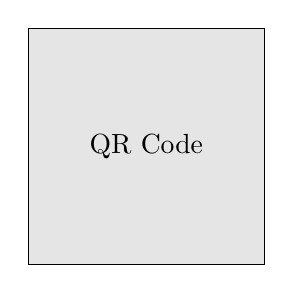
\begin{tikzpicture}
        \node[draw,fill=gray!20,minimum width=3cm,minimum height=3cm] {QR Code};
    \end{tikzpicture}
    
    \vspace{0.5em}
    扫码获取演讲资料
\end{frame}

\end{document}
